% $Header: /cvsroot/latex-beamer/latex-beamer/solutions/conference-talks/conference-ornate-20min.en.tex,v 1.6 2004/10/07 20:53:08 tantau Exp $

\documentclass{beamer}
%\documentclass[handout]{beamer}
%\usepackage{pgfpages}
%\pgfpagesuselayout{2 on 1}[a4paper,border shrink=5mm]

% This file is a solution template for:

% - Talk at a conference/colloquium.
% - Talk length is about 20min.
% - Style is ornate.



% Copyright 2004 by Till Tantau <tantau@users.sourceforge.net>.
%
% In principle, this file can be redistributed and/or modified under
% the terms of the GNU Public License, version 2.
%
% However, this file is supposed to be a template to be modified
% for your own needs. For this reason, if you use this file as a
% template and not specifically distribute it as part of a another
% package/program, I grant the extra permission to freely copy and
% modify this file as you see fit and even to delete this copyright
% notice.


\mode<presentation>
{
%  \usetheme{Warsaw}
%  \usetheme{Boadilla}
%  \usetheme{Goettingen}
%  \usetheme{Hannover}
%  \usetheme{Madrid}
%  \usetheme{Marburg}
%  \usetheme{Montpellier}
%  \usetheme{Pittsburgh}
  \usetheme{Hawke}
  % or ...

  \setbeamercovered{transparent}
  % or whatever (possibly just delete it)
}


\usepackage[english]{babel}
% or whatever

\usepackage[latin1]{inputenc}
% or whatever

\usepackage{times}
\usepackage[T1]{fontenc}
% Or whatever. Note that the encoding and the font should match. If T1
% does not look nice, try deleting the line with the fontenc.

\usepackage{multimedia}


%%%%%%
% My Commands
%%%%%%

\newcommand{\ml}{{\sc matlab}}
\newcommand{\bb}{{\boldsymbol{b}}}
\newcommand{\bx}{{\boldsymbol{x}}}
\newcommand{\by}{{\boldsymbol{y}}}
\newcommand{\bfm}[1]{{\boldsymbol{#1}}}
\newcommand{\oda}[2]{\frac{\text{d}{#1}}{\text{d}{#2}}}
\newcommand{\pda}[2]{\frac{\partial{#1}}{\partial{#2}}}
\newcommand{\pdb}[2]{\frac{\partial^2{#1}}{\partial{#2}^2}}
\newcommand{\pdc}[3]{\frac{\partial^2{#1}}{\partial{#2}\partial{#3}}}


%%%%

\title[Lecture 26] % (optional, use only with long paper titles)
{Lecture 26 - Multilevel Methods}

% \subtitle
% {Include Only If Paper Has a Subtitle}

\author[I. Hawke] % (optional, use only with lots of authors)
{I.~Hawke}
% - Give the names in the same order as the appear in the paper.
% - Use the \inst{?} command only if the authors have different
%   affiliation.

\institute[University of Southampton] % (optional, but mostly needed)
{
%  \inst{1}%
  School of Mathematics, \\
  University of Southampton, UK
}
% - Use the \inst command only if there are several affiliations.
% - Keep it simple, no one is interested in your street address.

\date[Semester 1] % (optional, should be abbreviation of conference name)
{MATH3018/6141, Semester 1}
% - Either use conference name or its abbreviation.
% - Not really informative to the audience, more for people (including
%   yourself) who are reading the slides online

\subject{Numerical methods}
% This is only inserted into the PDF information catalog. Can be left
% out.



% If you have a file called "university-logo-filename.xxx", where xxx
% is a graphic format that can be processed by latex or pdflatex,
% resp., then you can add a logo as follows:

\pgfdeclareimage[height=0.5cm]{university-logo}{mathematics_7469}
\logo{\pgfuseimage{university-logo}}



% Delete this, if you do not want the table of contents to pop up at
% the beginning of each subsection:
%  \AtBeginSubsection[]
%  {
%    \begin{frame}<beamer>
%      \frametitle{Outline}
%      \tableofcontents[currentsection,currentsubsection]
%    \end{frame}
%  }
\AtBeginSection[]
{
  \begin{frame}<beamer>
    \frametitle{Outline}
    \tableofcontents[currentsection]
  \end{frame}
}


% If you wish to uncover everything in a step-wise fashion, uncomment
% the following command:

%\beamerdefaultoverlayspecification{<+->}


\begin{document}

\begin{frame}
  \titlepage
\end{frame}

\section{Multilevel methods for PDEs}


\begin{frame}
  \frametitle{Partial differential equations}

  Partial differential equations (PDEs) involve derivatives of
  functions of more than one variable, say $u(x, y)$ or $y(t,
  x)$. Hence more complex behaviour and more interesting
  physics. \pause

  \vspace{1ex}

  Problem with standard methods: accuracy depends on $h$, hence
  inversely on $N$. \pause Improving accuracy is at least an $N^2$
  problem; increasing the dimension makes matters worse ($N^{d+1}$),
  and more accurate spectral methods are even more expensive. \pause

  \vspace{1ex}

  Saw with quadrature and IVPs that a careful choice of grid could
  improve matters. Also true for PDEs, but again must treat
  evolutionary and elliptic problems separately.

\end{frame}

\section{Adaptive Mesh Refinement}

\begin{frame}
  \frametitle{Grid locations}

  \begin{columns}
    \begin{column}{0.55\textwidth}
      Have considered only fixed, uniformly spaced grids. Easy to use
      but waste grid points in uninteresting areas. \pause An uneven
      grid removes waste, but complicates the algorithm and is
      difficult to generalize. \pause

      \vspace{1ex}

      Instead a number of grids of varying resolution can be used, all
      evenly spaced; this is \emph{mesh refinement}. \pause If the grid
      structure varies in time, this is \emph{adaptive} mesh
      refinement.
    \end{column}
    \begin{column}{0.45\textwidth}
      \begin{center}
        \includegraphics<1|handout:0>[width=\textwidth]{figures/Grids_Uni.png}
        \includegraphics<2|handout:1>[width=\textwidth]{figures/Grids_Uneven1.png}
        \includegraphics<3-|handout:2>[width=\textwidth]{figures/Grids_AMR1.png}
      \end{center}
    \end{column}
  \end{columns}

\end{frame}

\begin{frame}
  \frametitle{Evolution and the CFL condition}

  \begin{center}
    \includegraphics<1|handout:0>[width=0.9\textwidth]{figures/Grid1}
    \includegraphics<2|handout:0>[width=0.9\textwidth]{figures/Grid3a}
    \includegraphics<3|handout:0>[width=0.9\textwidth]{figures/Grid_AMR1}
    \includegraphics<4|handout:1>[width=0.9\textwidth]{figures/Grid_AMR2}
  \end{center}
  All grids are equally spaced as before. \pause Therefore timestep
  must obey CFL condition. \pause When using AMR introduce refined
  grids locally to improve accuracy.  \pause Therefore the CFL
  condition requires reducing timestep \emph{only on refined grid}.

\end{frame}

\begin{frame}
  \frametitle{Inter-grid operations}

  \begin{columns}
    \begin{column}{0.5\textwidth}
      Evolution for each grid is independent in interior. \pause
      However, boundaries of finer grids lie in interior of the
      coarse; boundary conditions for fine grid require
      interpolation. \pause

      \vspace{1ex}

      Also couple coarse grid to fine. \pause Update coarse grid from
      fine points wherever possible.
    \end{column}
    \begin{column}{0.5\textwidth}
      \includegraphics<1-2|handout:0>[width=\textwidth]{figures/Grids_AMR1}
      \includegraphics<3-|handout:1>[width=\textwidth]{figures/Grids_AMR2}
    \end{column}
  \end{columns}

\end{frame}

\begin{frame}
  \frametitle{Error indicators}

  AMR improves efficiency when grids are located correctly. \pause
  Need to choose where the grids are to be located. \pause This choice
  must depend on the data and the \emph{local} numerical
  accuracy. \pause

  \vspace{1ex}

  One local error estimate is Richardson extrapolation. \pause Given
  \emph{two} approximations to $\by$ at resolutions $h$, $2 h$, the
  computable error is
  \begin{equation*}
    \bfm{E}_{2 h} \equiv \frac{|\by_{2 h} - \by_h|}{2^s - 1}.
  \end{equation*}
  $s$ is convergence rate of algorithm. \pause

  \vspace{1ex}

  Now have an error estimate at each grid point; ``just'' choose finer
  grids to cover points where $E_{2 h} > \text{tolerance}$
  (non-trivial in many dimensions).


\end{frame}

\begin{frame}
  \frametitle{Colella-Woodward test}

  \begin{columns}
    \begin{column}{0.5\textwidth}
      Difficult test involving blast waves. Use Euler equations,
      discontinuous initial data in a ``closed tube'', and an
      upwind-type method. \pause

      \vspace{1ex}

      Shocks propagate, \pause bouncing off the ends of the tube \pause
      and interacting \pause in a complex fashion. \pause

      \vspace{1ex}

      Grid adapts to the flow; resolution equivalent to a uniform grid
      of 80,000 points but only 4,000 are ever required.
    \end{column}
    \begin{column}{0.5\textwidth}
      \begin{overlayarea}{\textwidth}{0.9\textheight}
        \only<1|handout:0>
        {
          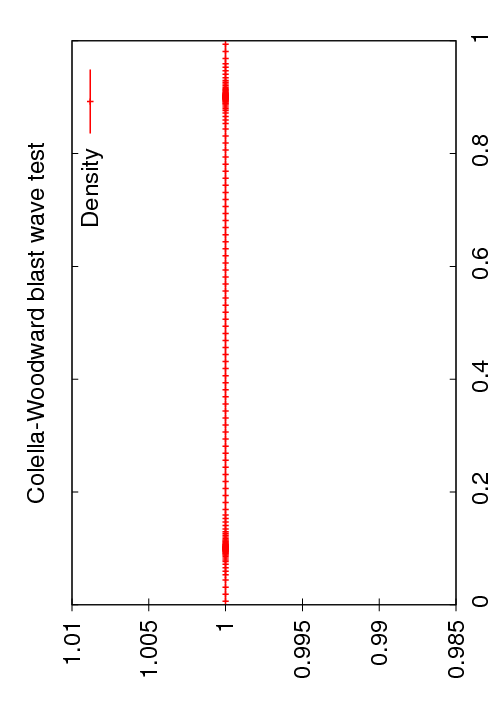
\includegraphics[angle=-90,width=0.9\textwidth]{figures/AMR_Density_0}\\
          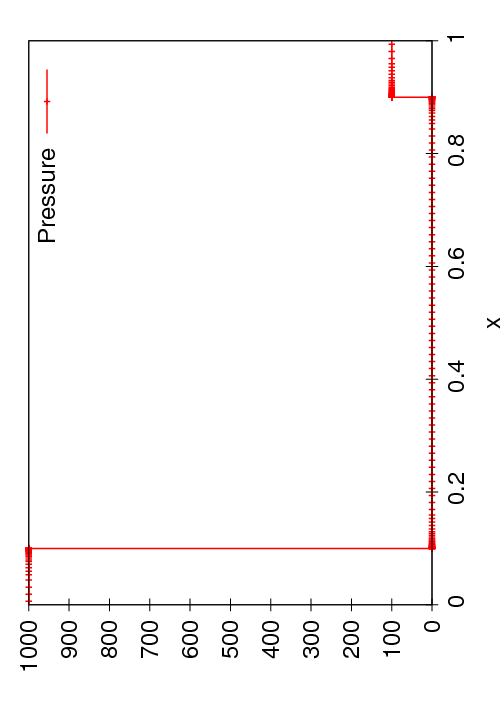
\includegraphics[angle=-90,width=0.9\textwidth]{figures/AMR_Pressure_0}
        }
        \only<2|handout:0>
        {
          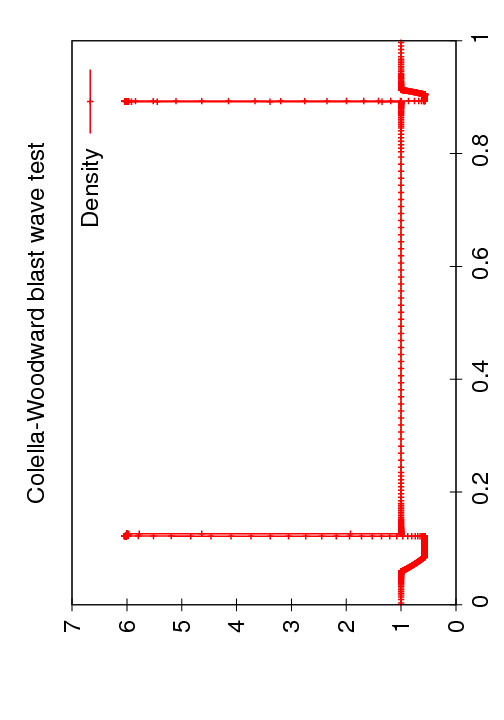
\includegraphics[angle=-90,width=0.9\textwidth]{figures/AMR_Density_10}\\
          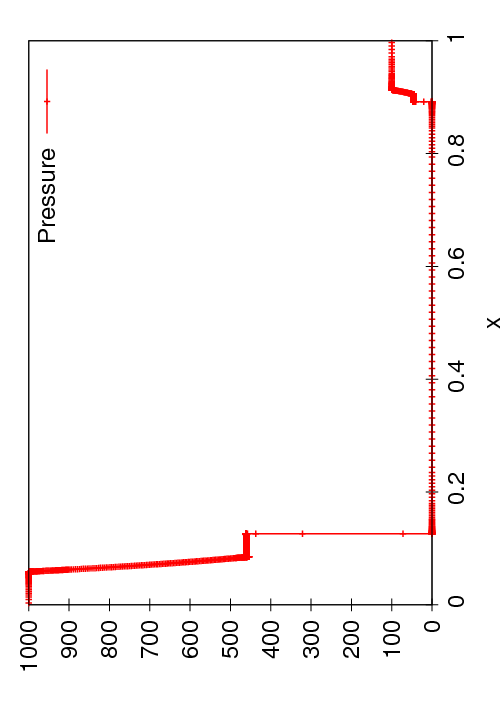
\includegraphics[angle=-90,width=0.9\textwidth]{figures/AMR_Pressure_10}
        }
        \only<3|handout:0>
        {
          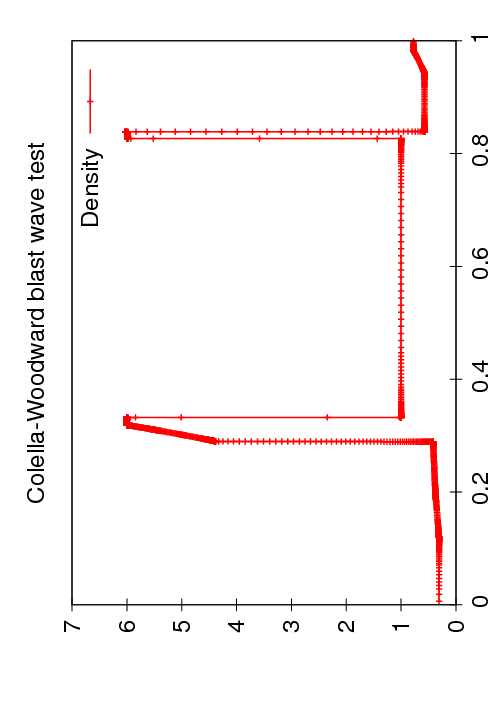
\includegraphics[angle=-90,width=0.9\textwidth]{figures/AMR_Density_100}\\
          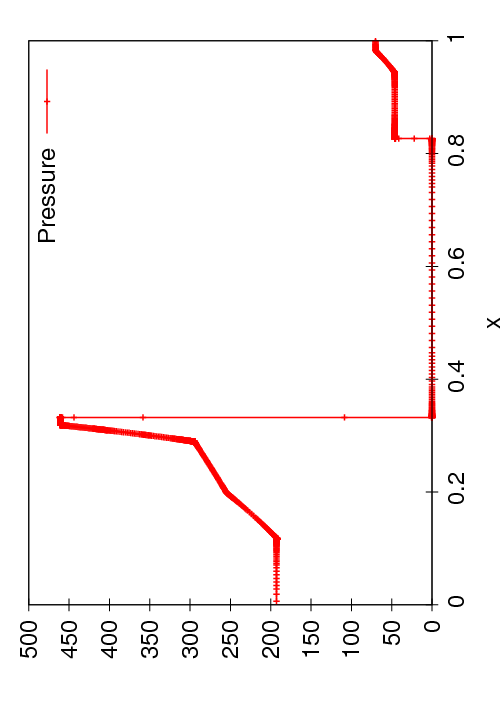
\includegraphics[angle=-90,width=0.9\textwidth]{figures/AMR_Pressure_100}
        }
        \only<4|handout:0>
        {
          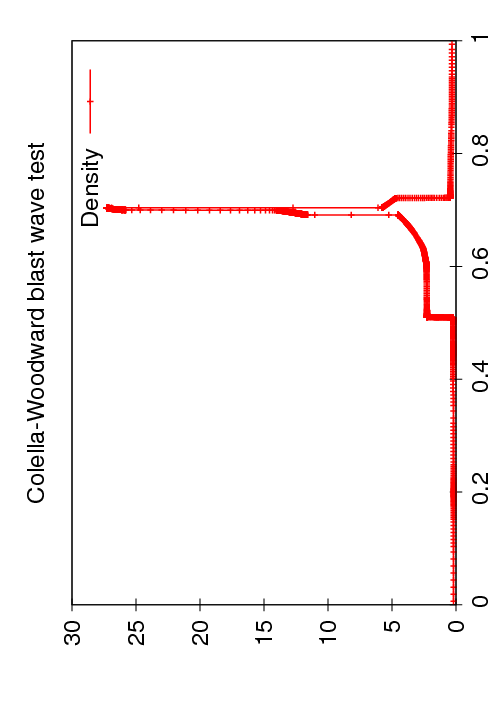
\includegraphics[angle=-90,width=0.9\textwidth]{figures/AMR_Density_250}\\
          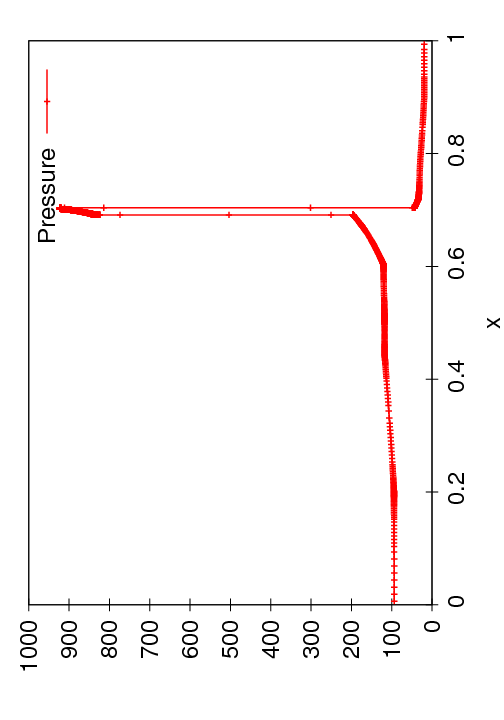
\includegraphics[angle=-90,width=0.9\textwidth]{figures/AMR_Pressure_250}
        }
        \only<5-|handout:1>
        {
          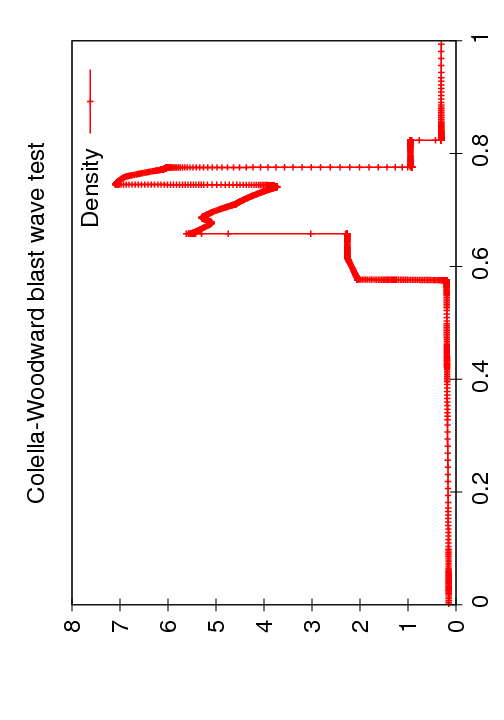
\includegraphics[angle=-90,width=0.9\textwidth]{figures/AMR_Density_300}\\
          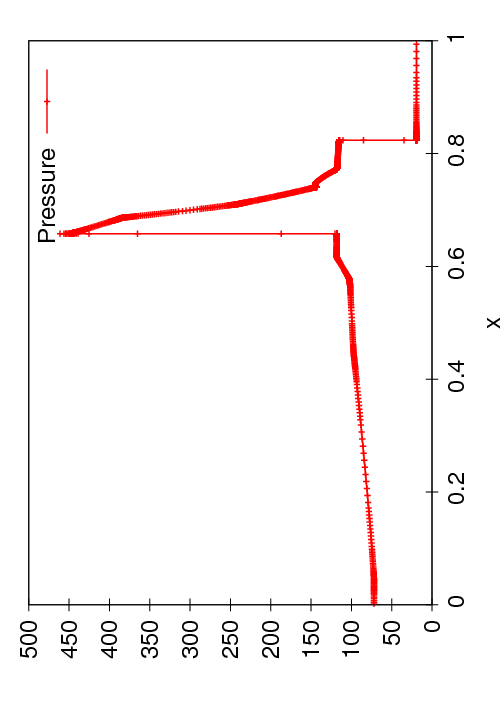
\includegraphics[angle=-90,width=0.9\textwidth]{figures/AMR_Pressure_300}
        }
      \end{overlayarea}
    \end{column}
  \end{columns}

\end{frame}

\section{Multigrid methods}


\begin{frame}
  \frametitle{Elliptic PDEs}

  When using finite differences to solve elliptic equations, typically
  use an iterative solver for resulting linear system. \pause

  \vspace{1ex}

  Universal features of iterative solvers: \pause
  \begin{enumerate}
  \item Accuracy of initial guess has direct impact on
    absolute error. \pause
  \item Smoothness of data has direct impact on convergence rate of
    error.
  \end{enumerate} \pause

  \vspace{1ex}

  The \emph{multigrid} method greatly speeds convergence by using
  different grids and aliasing.

\end{frame}

\begin{frame}
  \frametitle{Initial guess}

  Want best possible initial guess. Best possible guess: solution
  itself. Therefore, want to start from solution. \pause

  \vspace{1ex}

  Obviously impossible. However, could start from \emph{approximate}
  solution. \pause Want solution $\by$ on grid resolution $h$,
  $\by^h$. Then compute solution on a coarser grid, $\by^{2 h}$ say,
  and use as initial guess. \pause Assume we have an \emph{intergrid
    operator} that takes $\by$ from fine grid to coarse. Write as
  \begin{equation*}
    \by^{2 h} = I^{2 h}_{h} \by^{h}.
  \end{equation*}\pause

  \vspace{1ex}

  To get coarse solution on fine grid, have to
  \emph{interpolate}. \pause Write as an operator
  \begin{equation*}
    \by^{h} = I^{h}_{2 h} \by^{2 h}.
  \end{equation*}

\end{frame}

\begin{frame}
  \frametitle{Recursion}

  Finding initial guess from coarser solution $\by^{2 h}$ postpones
  the problem; still have to solve the coarser problem. \pause Use
  same iterative method on coarser grid, so use same approach for
  initial guess: coarsen again. \pause

  \vspace{1ex}

  Apply technique \emph{recursively}, and assume grid has a suitable
  number of points, say $N = 2^k$. Eventually left with a linear
  system on a very small grid, i.e.\ $N = 1$. Can be done
  directly. \pause

  \vspace{1ex}

  Having found \emph{an} initial guess on a coarse grid, use
  interpolation operator $I^{h}_{2 h}$ to move to a finer grid, and
  then solve, to get the accurate initial guess that required.

\end{frame}

\begin{frame}
  \frametitle{Frequency effects}

  \begin{columns}
    \begin{column}{0.5\textwidth}
      Smoothness of initial data changes convergence speed. Example:
      model problem
      \begin{equation*}
        u'' = 0, \,\, u(0) = 0 = u(1)
      \end{equation*}
      has trivial solution. \pause Investigate frequency dependence
      using weighted Jacobi method with initial guess
      \begin{equation*}
        u^{(0)}_i = \sin \left( \frac{i k \pi}{N} \right)
      \end{equation*}
      ($N$ gridpoints, $k$ controls frequency).
    \end{column}
    \begin{column}{0.5\textwidth}
      \includegraphics<2|handout:0>[width=\textwidth]{figures/Smoothing1a}
      \includegraphics<3-|handout:1>[width=\textwidth]{figures/Smoothing1b}
    \end{column}
  \end{columns}

\end{frame}

\begin{frame}
  \frametitle{Frequency effects: 2}

  \begin{columns}
    \begin{column}{0.4\textwidth}
      Convergence rate increases with $k$. \pause

      \vspace{1ex}

      Has dramatic effect on the number of iterations required for
      convergence. After a few iterations, error dominated by ``low''
      frequency features that appear smooth on the grid.
    \end{column}
    \begin{column}{0.6\textwidth}
      \includegraphics<1|handout:0>[width=\textwidth]{figures/Smoothing2}
      \includegraphics<2-|handout:1>[width=\textwidth]{figures/Smoothing3}
    \end{column}
  \end{columns}

\end{frame}

\begin{frame}
  \frametitle{Aliasing and frequency}

  \begin{columns}
    \begin{column}{0.45\textwidth}
      Problem of ``low'' frequencies not
      insurmountable. \emph{Aliasing} effect: high and low frequency
      wave can appear equivalent if the grid resolution is ``too
      coarse''. \pause

      \vspace{1ex}

      Take advantage: move to a coarser grid $\rightarrow$ error
      appears to be made of higher frequencies $\rightarrow$ converge
      faster!
    \end{column}
    \begin{column}{0.54\textwidth}
      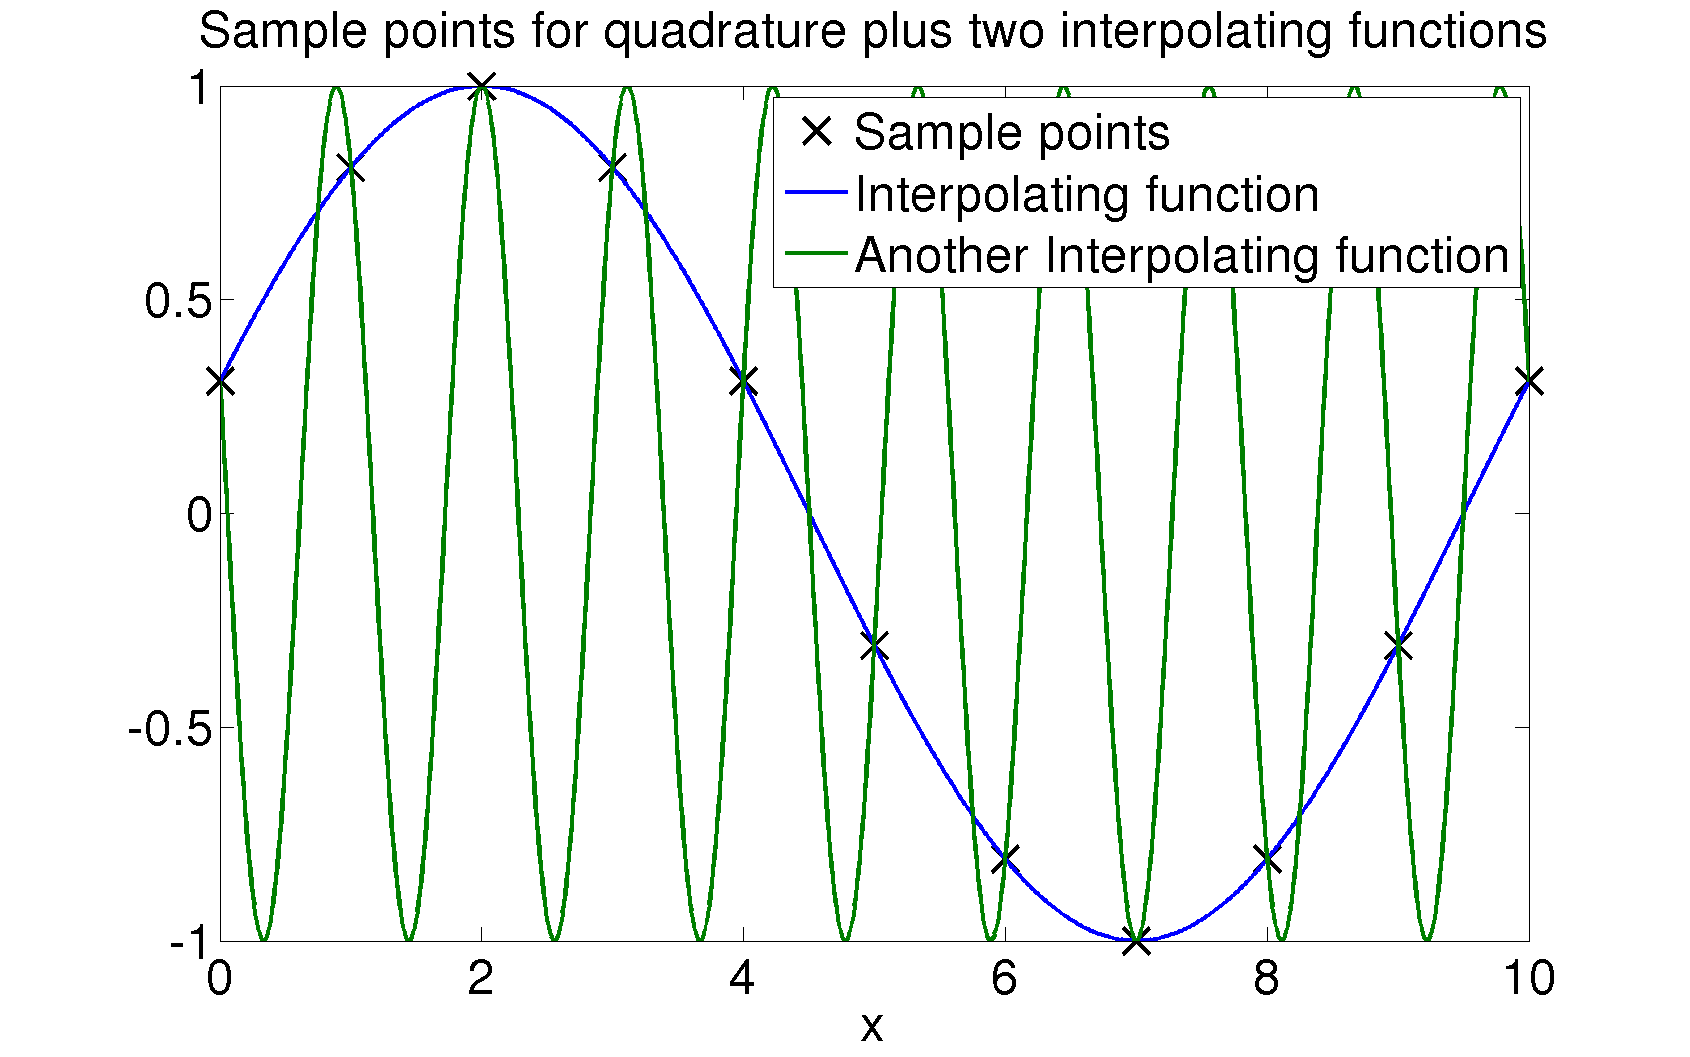
\includegraphics[width=\textwidth]{figures/QuadAliasing4}
    \end{column}
  \end{columns}

\end{frame}

\begin{frame}
  \frametitle{The multigrid V-cycle (MV) algorithm}

  Denote grid, spacing $h$ as $\Omega^h$. Denote algorithm starting at
  that spacing $MV^h (\by^h, \bfm{f}^h)$, where equation is
  \begin{equation*}
    {\cal L} \by = \bfm{f}.
  \end{equation*}

  \begin{enumerate}
  \item Relax $\nu_1$ times on $\Omega^h$. \pause
  \item If $\Omega^h$  coarsest grid, go to step 4. \pause Else
    restrict to coarse grid to set
    \begin{align*}
      \bfm{f}^{2 h} &\leftarrow I^{2 h}_h \left( \bfm{f}^h - A^h \by^h
      \right) \\
      \by^{2 h} & \leftarrow 0 \\
      \by^{2 h} & \leftarrow MV^{2 h} (\by^{2 h}, \bfm{f}^{2 h})
    \end{align*} \pause \vspace{-2ex}
  \item Then correct (interpolate) to set
    \begin{equation*}
      \by^h \leftarrow \by^h + I^h_{2 h} \by^{2 h}.
    \end{equation*} \pause \vspace{-2ex}
  \item Relax $\nu_2$ times on $\Omega^h$.
  \end{enumerate}

\end{frame}

\begin{frame}
  \frametitle{Cycles and cycles}

  \begin{columns}
    \begin{column}{0.45\textwidth}
      Previous algorithm called the V-cycle because of order of
      relaxation steps on different grids. \pause

      \vspace{1ex}

      More effective algorithms include the W-cycle \pause or the full
      multigrid V-cycle (FMV). Based around same ideas and essentially
      include V-cycles within themselves.
    \end{column}
    \begin{column}{0.55\textwidth}
      \includegraphics<1|handout:0>[width=\textwidth]{figures/VCycle}
      \includegraphics<2|handout:1>[width=\textwidth]{figures/WCycle}
      \includegraphics<3-|handout:0>[width=\textwidth]{figures/FMVCycle}
    \end{column}
  \end{columns}

\end{frame}

\section{Summary}

\subsection{Summary}

\begin{frame}
  \frametitle{Summary}

  \begin{itemize}
  \item In higher dimensions the basic algorithms applied to single,
    uniformly spaced grids are not competitive.
  \item For evolutionary equations one technique is Adaptive Mesh
    Refinement (AMR):
    \begin{itemize}
    \item Finer grids are added only where extra accuracy is required
    \item The grids are evolved independently based on the stability
      condition of the evolution algorithm
    \item Fine grids need interpolation from the coarse grids for
      boundary conditions
    \item Coarse grids need restriction from the fine for accuracy
    \end{itemize}
  \item For elliptic equations multigrid is very popular:
    \begin{itemize}
    \item By cycling through grids with different resolutions the best
      balance between accuracy and efficiency is found
    \item The coarse grids are better at damping low frequency, and
      rapidly find accurate guesses for the fine grids
    \end{itemize}
  \item Multigrid is much more robust than spectral methods, but does
    not give the same level of accuracy.
  \end{itemize}

\end{frame}

\end{document}



%%% Local Variables:
%%% mode: latex
%%% TeX-master: t
%%% End:
